\begin{figure*}
\centering
\begin{subfigure}[h]{0.35\textwidth}
\caption{}
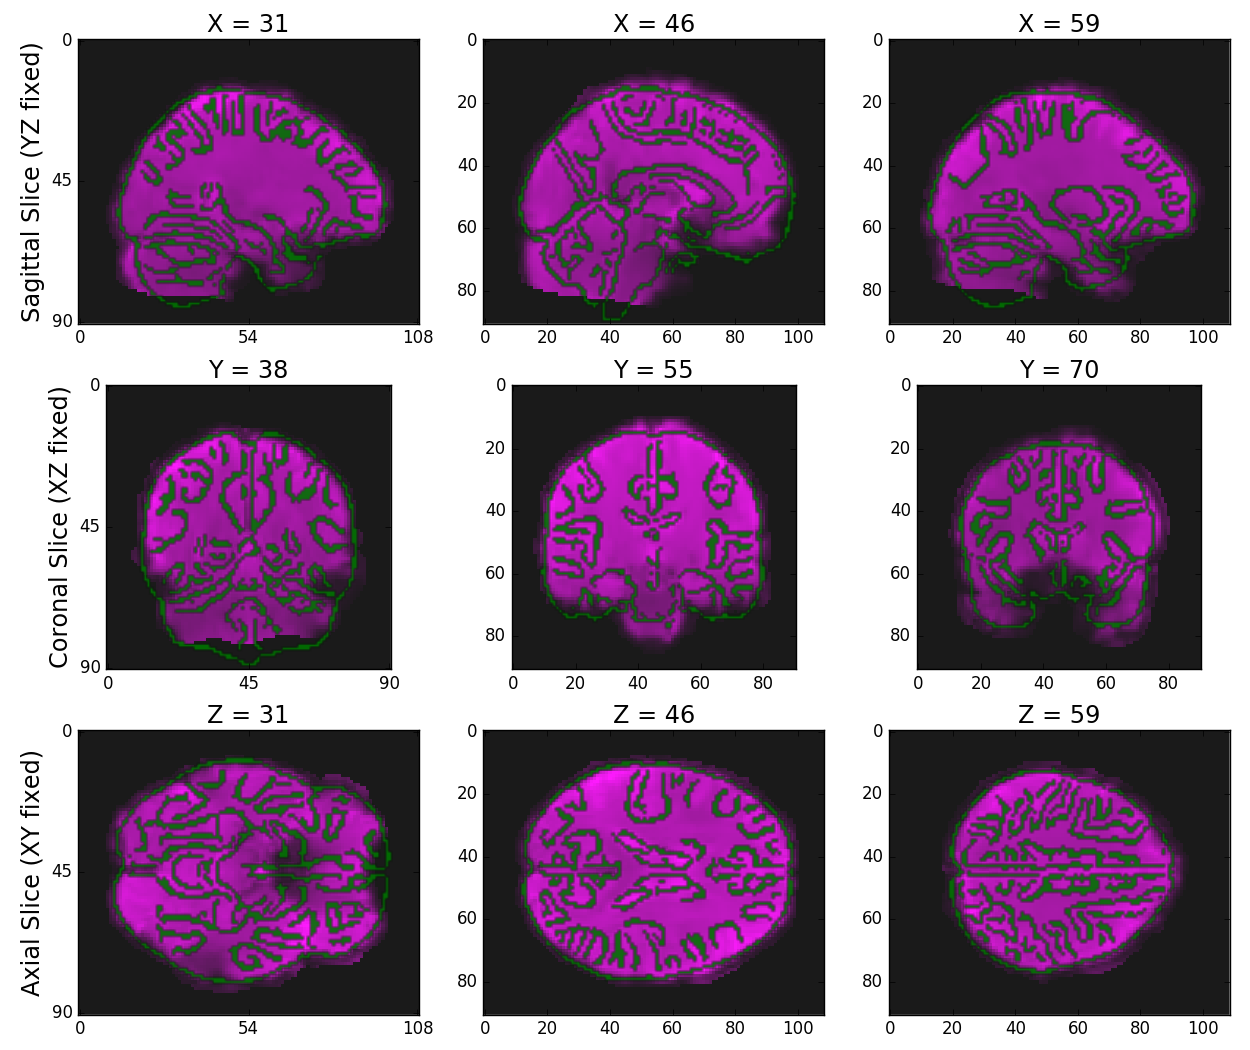
\includegraphics[width=\textwidth]{./qa_figs/fig_fmri_reg_epi2temp.png}
\label{fig:epi2tmp}
\end{subfigure}
\begin{subfigure}[h]{0.35\textwidth}
\caption{}
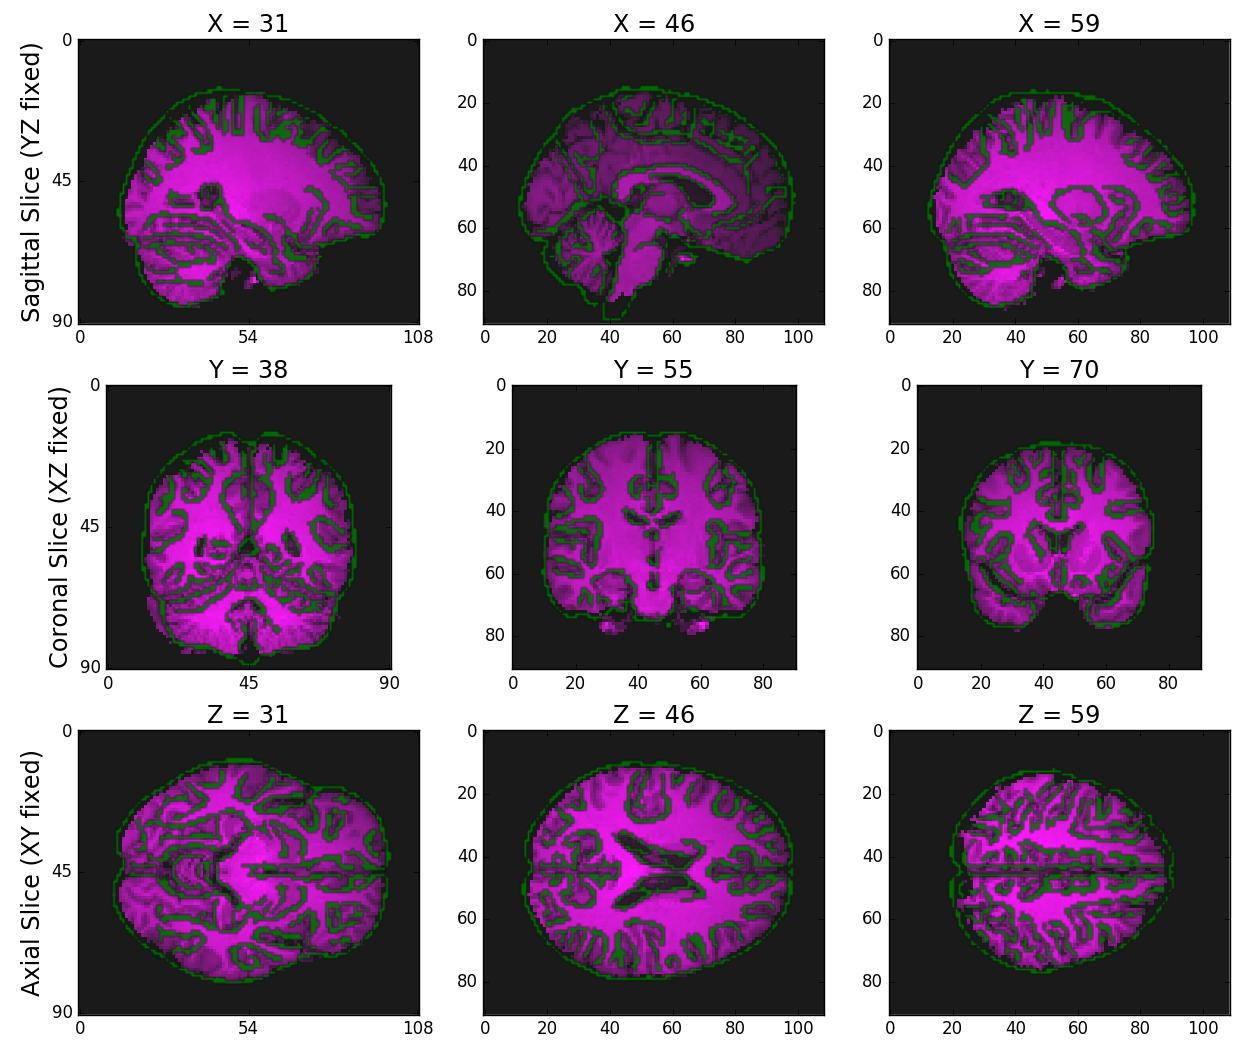
\includegraphics[width=\textwidth]{./qa_figs/fig_fmri_reg_t1w2temp.png}
\label{fig:t1w2tmp}
\end{subfigure}
\begin{subfigure}[h]{0.35\textwidth}
\caption{}
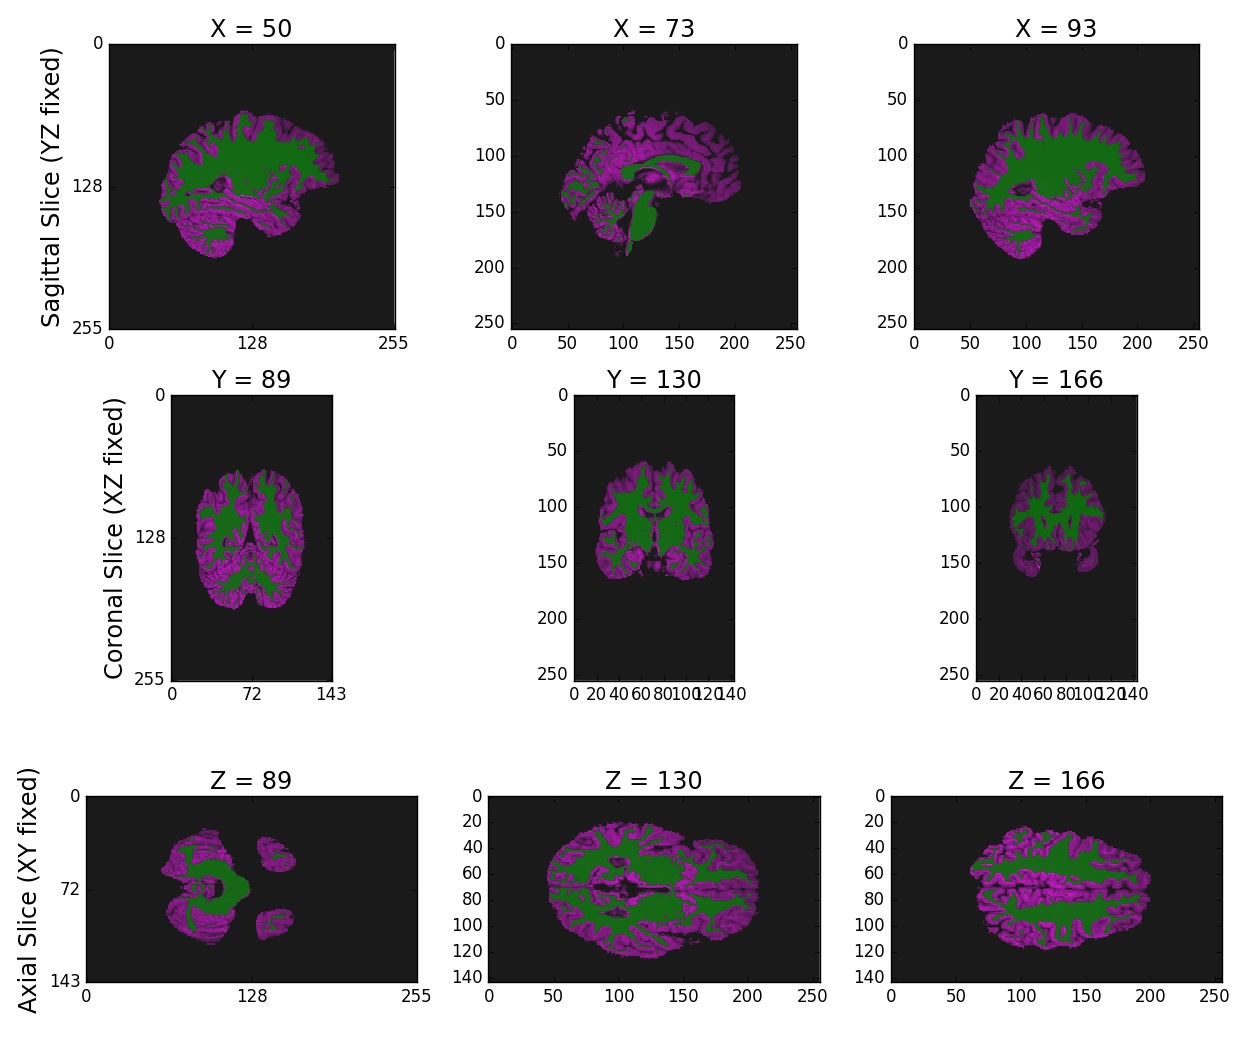
\includegraphics[width=\textwidth]{./qa_figs/fig_fmri_reg_t1w_wmm.png}
\label{fig:wmm}
\end{subfigure}
\begin{subfigure}[h]{0.35\textwidth}
\caption{}
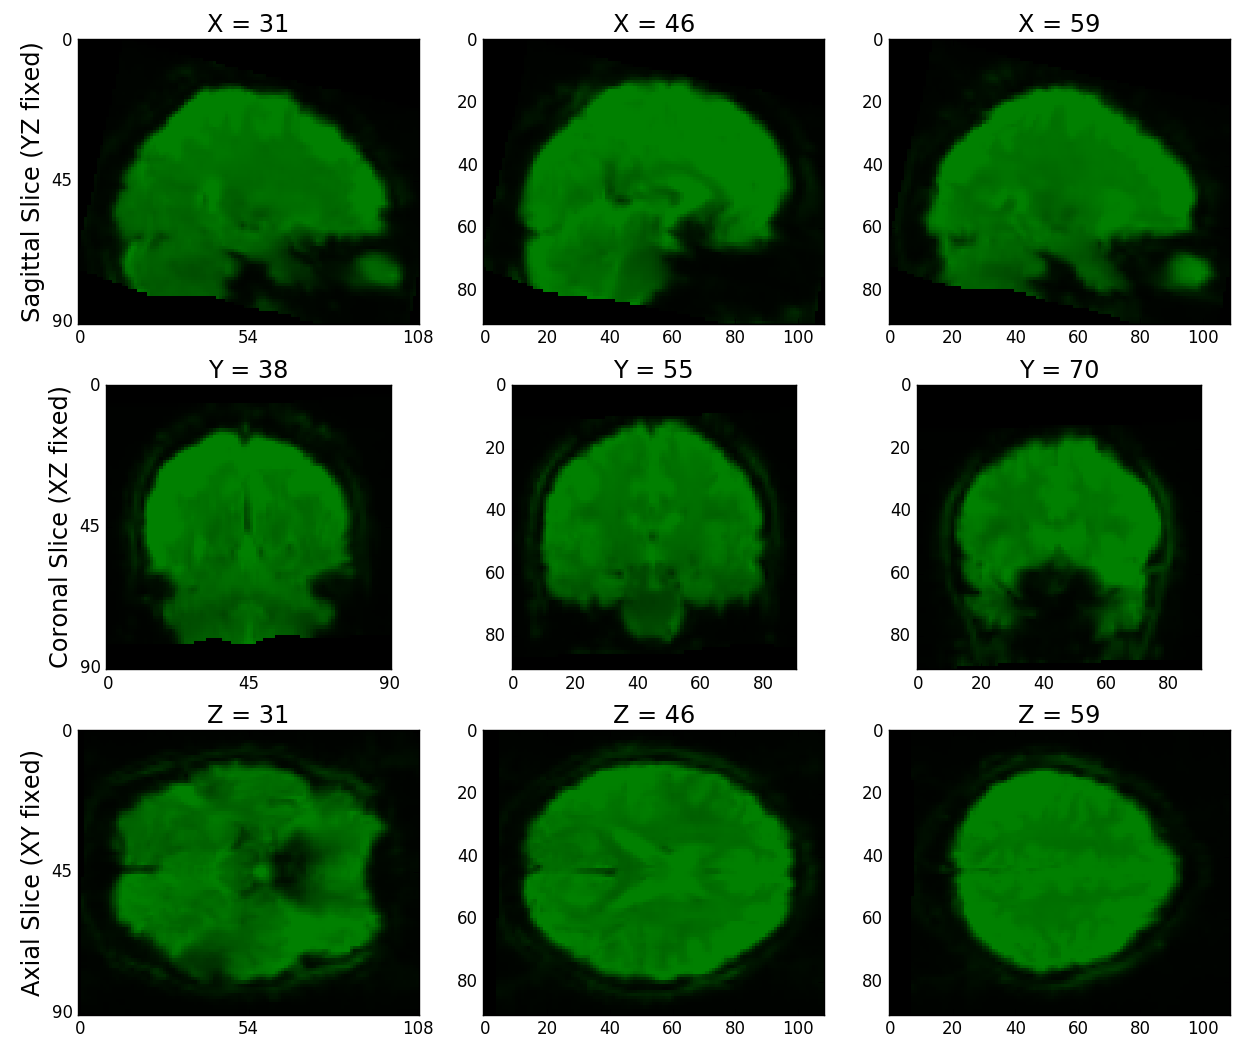
\includegraphics[width=\textwidth]{./qa_figs/fig_fmri_reg_mean.png}
\label{fig:fmean}
\end{subfigure}
\begin{subfigure}[h]{0.35\textwidth}
\caption{}
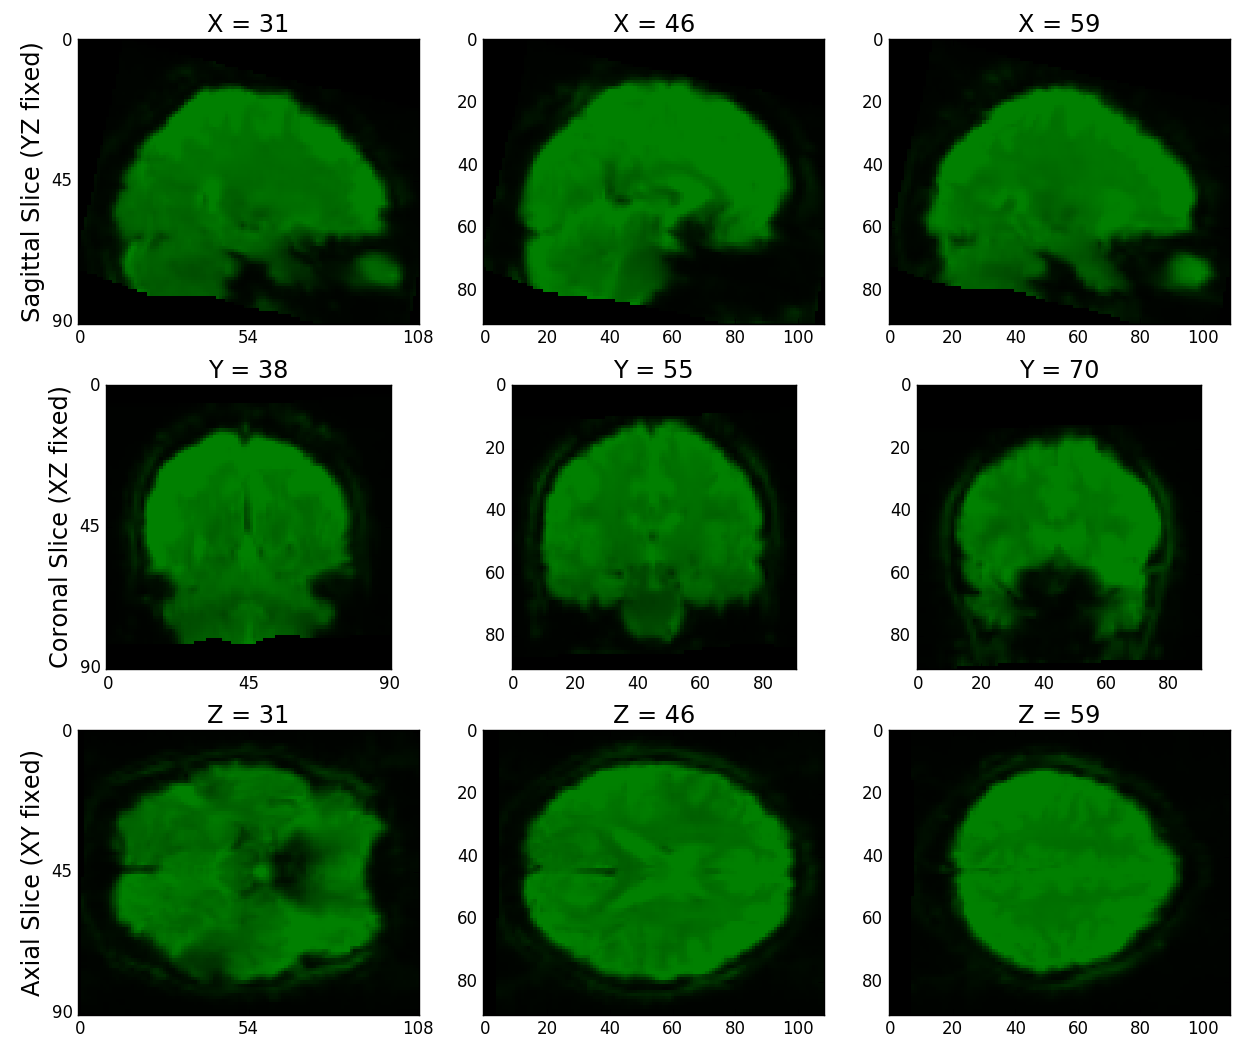
\includegraphics[width=\textwidth]{./qa_figs/fig_fmri_reg_snr.png}
\label{fig:snr}
\end{subfigure}
\begin{subfigure}[h]{0.35\textwidth}
\caption{}
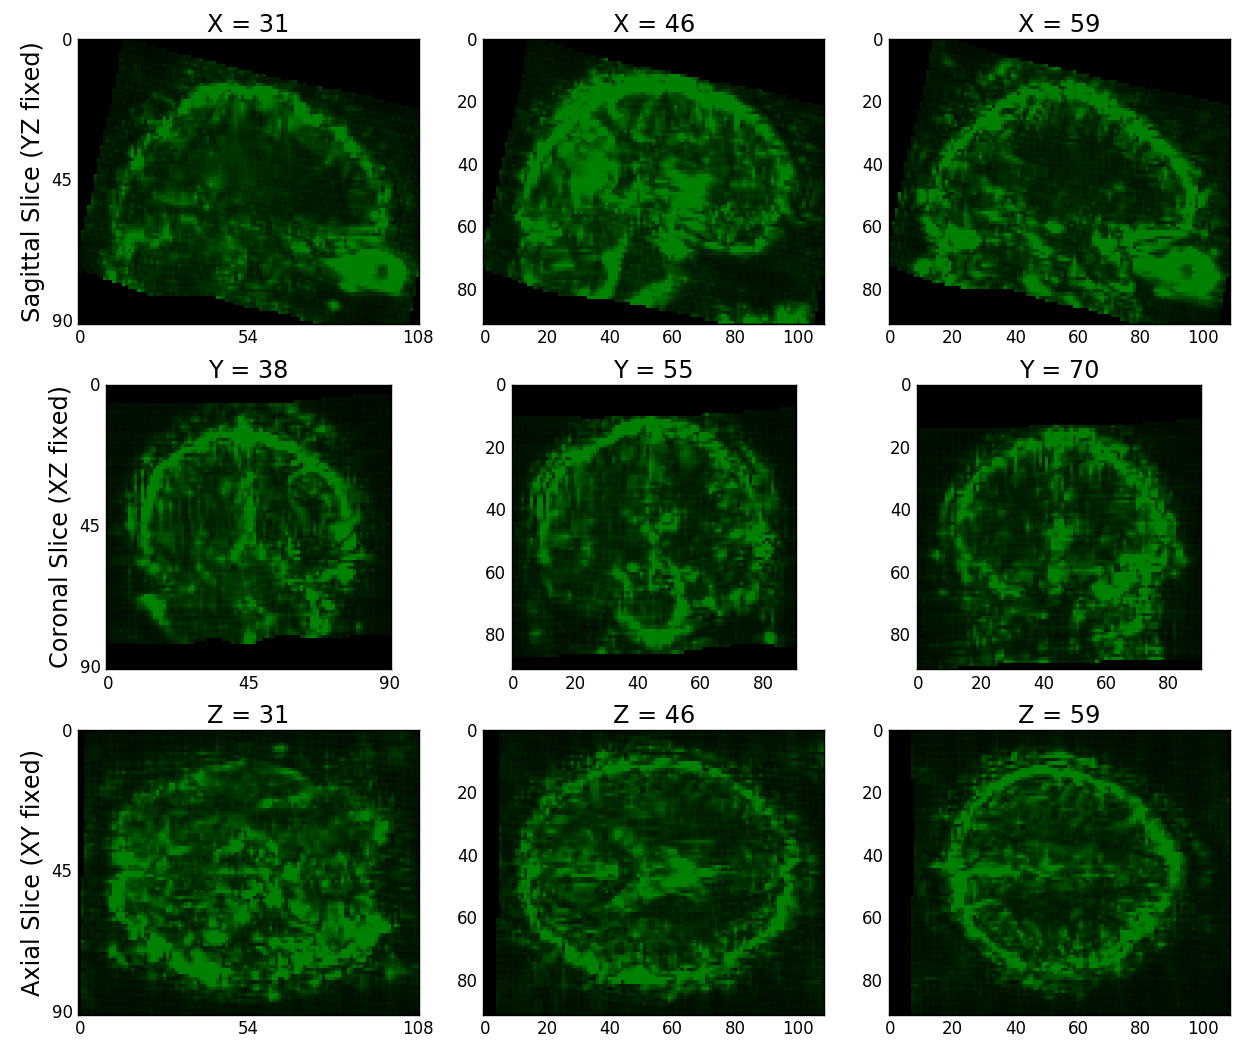
\includegraphics[width=\textwidth]{./qa_figs/fig_fmri_reg_cnr.png}
\label{fig:cnr}
\end{subfigure}
\caption{\textbf{\ndmgf~Registration QAX}. For registration, \ndmgf~ produces summary figures showing the preprocessed epi image overlaid on the t1w, the registered epi image overlaid on the template (\ref{fig:epi2tmp}), the registered t1w image overlaid on the template (\ref{fig:t1w2tmp}), the white-matter mask used in FLIRT-bbr (\ref{fig:wmm}), the voxelwise mean intensity (\ref{fig:mean}), the voxelwise signal-to-noise ratio (\ref{fig:snr}), and the voxelwise contrast-to-noise ratio (\ref{fig:cnr}).}
\label{fig:fmri_reg}
\end{figure*}